\documentclass[10pt]{beamer}
%\usepackage[utf8]{inputenc}
\usetheme{default}
\usepackage{xcolor}
\usepackage{graphicx}
\definecolor{backcolor}{HTML}{004586}
\definecolor{forecolor}{HTML}{FFFFFF}
\definecolor{ftcolor}{HTML}{FFF2CC}
\definecolor{sapienza}{HTML}{830029}

\newcommand{\printauthor}{Enrico Bassetti}

% ToC:
% - Parte 1: terremoti (slide Panizzi)
% - Parte 2: SeismoCloud

\setbeamertemplate{headline}
{
}

\setbeamertemplate{frametitle}
{
	\vskip-3pt
	\leavevmode
	\hbox{
		\begin{beamercolorbox}[wd=\paperwidth,ht=4ex,dp=1ex]{frametitle}
			$\vcenter{\hbox{
\includegraphics[keepaspectratio=true,height=40pt]{llg}}}$
			\raggedright\hspace*{2em}\large\insertframetitle
		\end{beamercolorbox}
	}
}
\setbeamertemplate{footline}
{
	\hbox{
		\begin{beamercolorbox}[wd=\paperwidth,ht=3.8ex,dp=3ex]{footline}
			\centering
			LD2016 @ Latina Linux Group
			\hspace{5em}
			\today
			\hspace{5em}
			Progetto SeismoCloud
			\hspace{5em}
			\printauthor
		\end{beamercolorbox}
	}
}


\setbeamercolor{normal text}{fg=forecolor}
\setbeamercolor{frametitle}{fg=ftcolor}
\setbeamercolor{footline}{fg=forecolor}
\setbeamercolor{background canvas}{bg=backcolor}
\setbeamercolor{item}{fg=white}

\beamertemplatenavigationsymbolsempty

\begin{document}

	\begin{frame}
		\frametitle{\hfill}
		
		\LARGE SeismoCloud		
		
	\end{frame}
	
	%%%%%%%%%%%%%%%%%%% PARTE 1
	
	\begin{frame}
		\frametitle{Parte 1}
		\LARGE Informazioni di base sui terremoti
	\end{frame}
	
	\begin{frame}
	\frametitle{I Terremoti}
	\begin{itemize}
	\item \textbf{Perché avvengono?}
		\begin{itemize}
			\item \pause Movimenti delle placche continentali
		\end{itemize}
	\item \textbf{Come avvengono?}
		\begin{itemize}
			\item \pause Le placche si muovono
			\item \pause L'attrito tra le placche non le fa muovere, ma genera tensione
			\item \pause Quando la tensione supera la resistenza: \textbf{terremoto!}
		\end{itemize}
	\end{itemize}
\end{frame}
\begin{frame}
	\frametitle{Placche planetarie}
	\hspace{1em}
	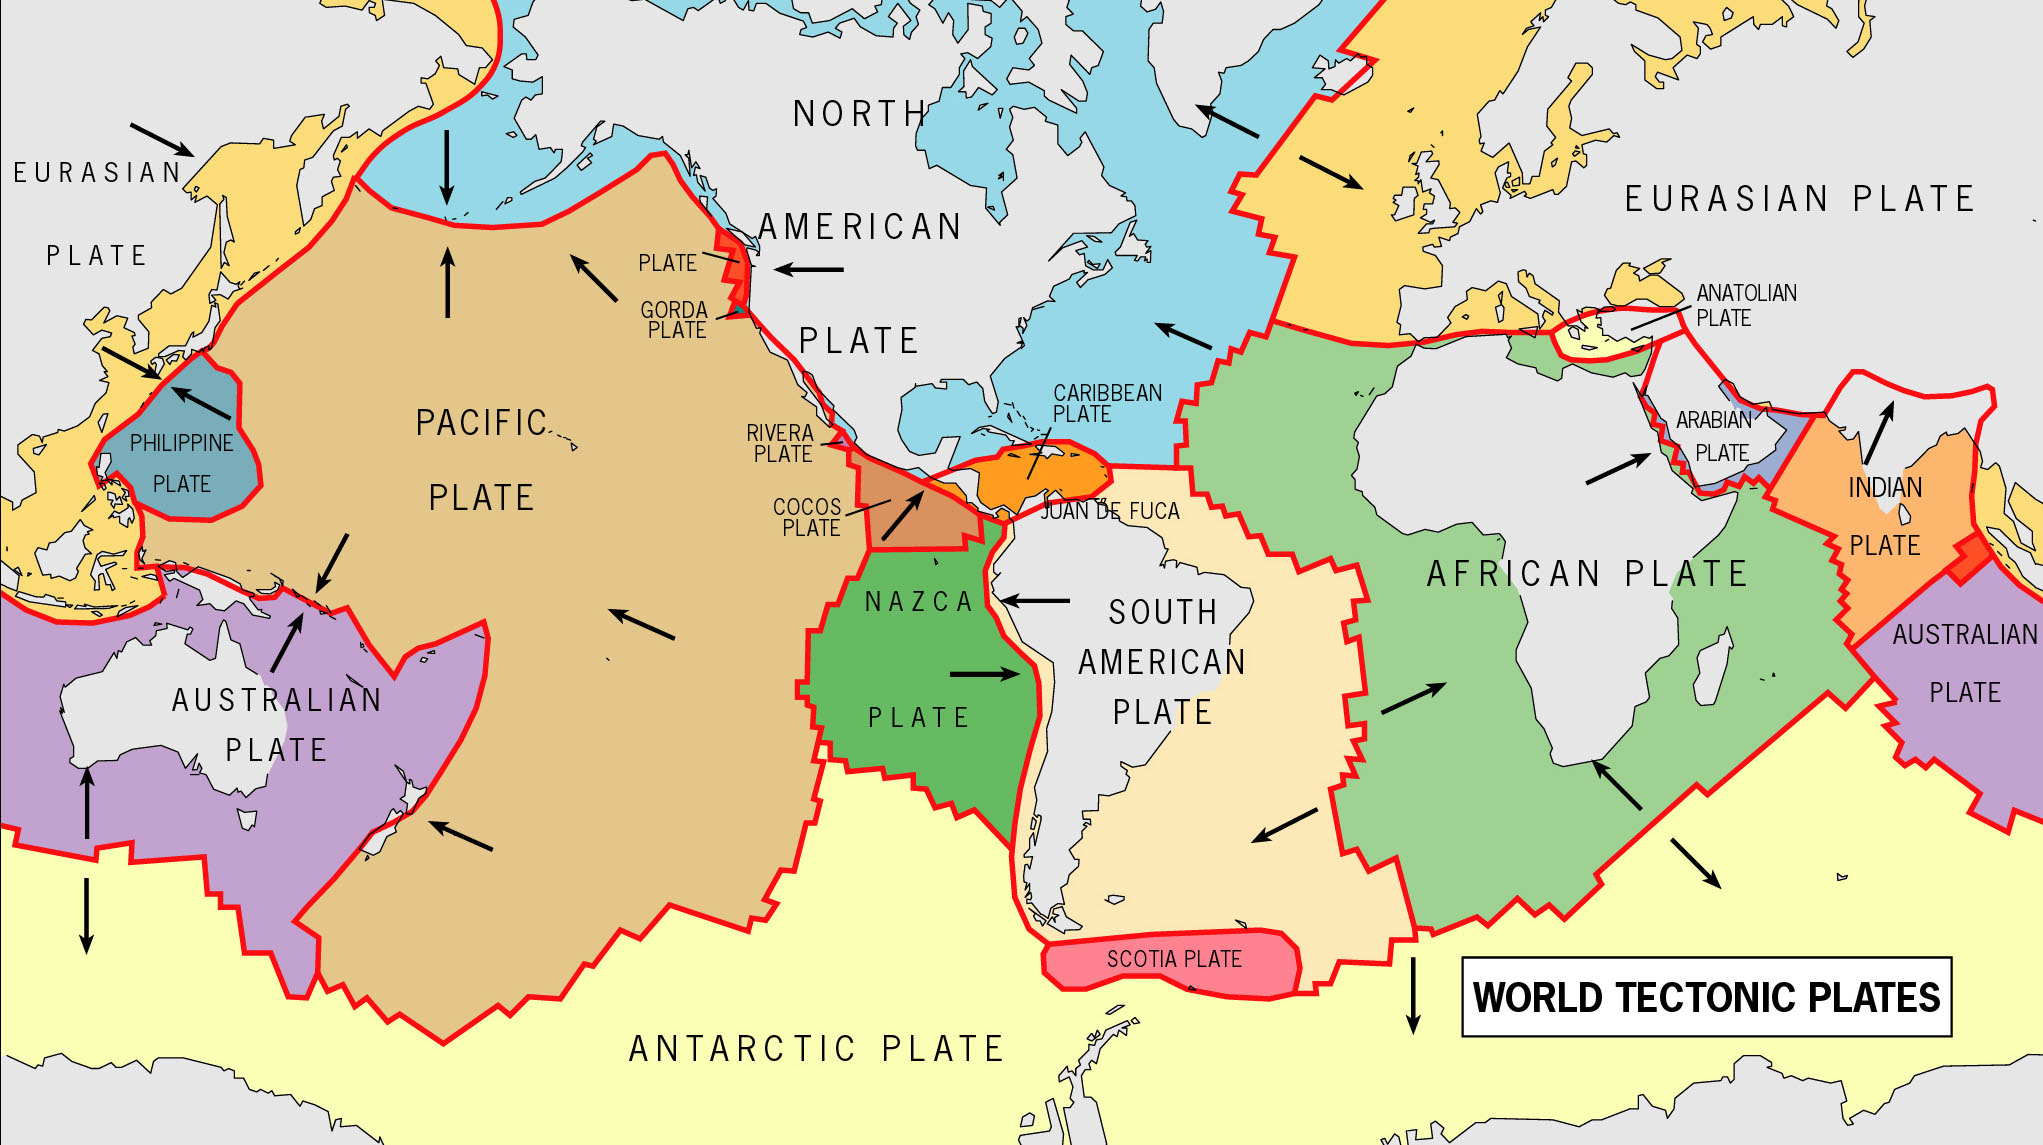
\includegraphics[keepaspectratio=true,width=0.8\paperwidth]{tectonic-plate}
\end{frame}
\begin{frame}
	\frametitle{Divisione dell'Italia nelle placche intercontinentali}
	\hspace{1em}
	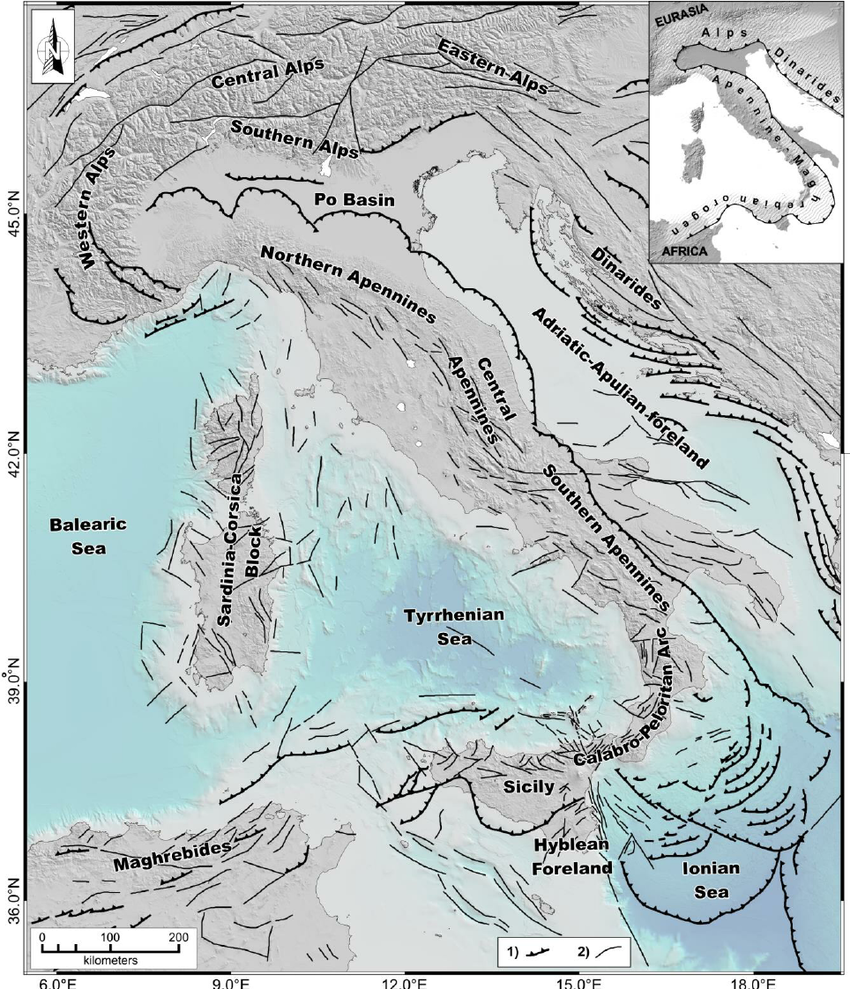
\includegraphics[keepaspectratio=true,height=0.8\paperheight]{italy-tectonic-map}
\end{frame}
	
	\begin{frame}
	\frametitle{Terminologia}
	\begin{itemize}
	\item \textbf{Ipocentro}: luogo di origine del terremoto
	\item \textbf{Epicentro}: proiezione dell'ipocentro in superficie
	\item \textbf{Faglia}: frattura tra due placche
	\item \textbf{Sismografo}: dispositivo analogico per la misurazione delle onde sismiche, \textit{non più in uso}
	\item \textbf{Sismometro}: sistema di misurazione digitale/elettronico del terremoto
	\end{itemize}
\end{frame}
\begin{frame}
	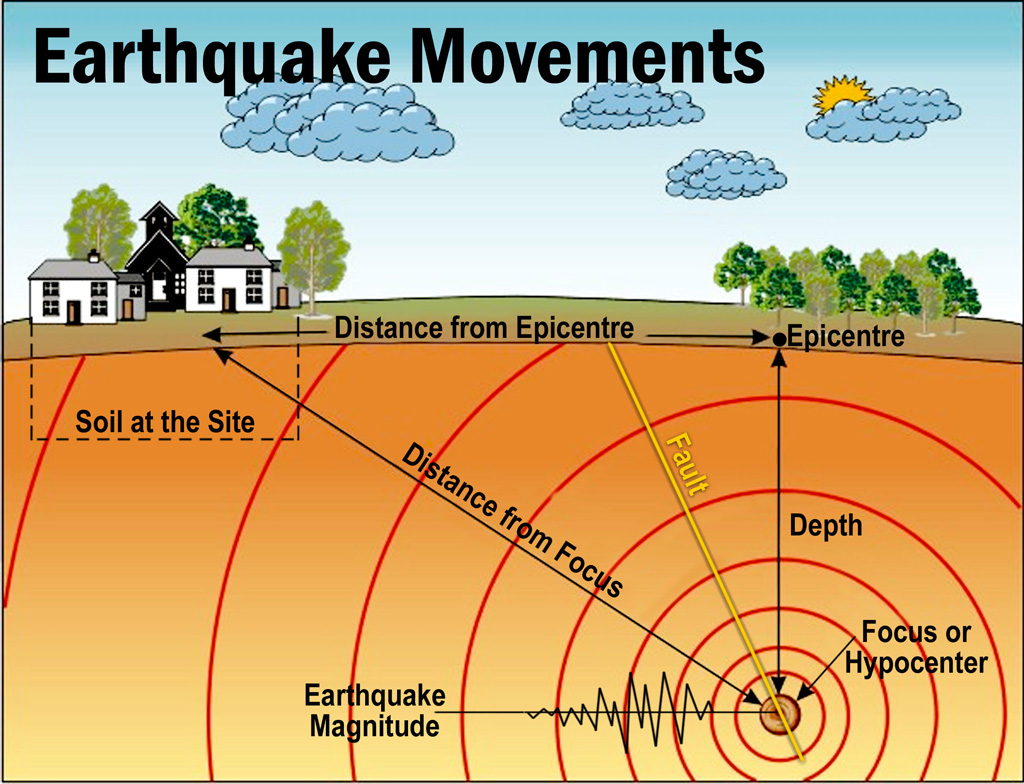
\includegraphics[keepaspectratio=true,width=0.8\paperwidth]{earthquake-points}
\end{frame}

	
	\begin{frame}
	\frametitle{Intensità e magnitudo}
	\begin{itemize}
	\item \textbf{Magnitudo Richter}
		\begin{itemize}
			\item Quantificare l'energia sprigionata dal terremoto
			\item Misurata solo con strumenti (sismometro)
		\end{itemize}
	\item<2-> \textbf{Intensità MCS} (Mercalli-Cancani-Sieberg)
		\begin{itemize}
			\item Quantifica i danni provocati dal terremoto
			\item Misurata con sopralluoghi e verifiche tecniche
			\item Dipende dal luogo e dalle tecniche costruttive
		\end{itemize}
	\end{itemize}
\end{frame}

	
	\begin{frame}
	\frametitle{I Terremoti}
	
	\LARGE Quanti terremoti ci sono ogni giorno?
	\pause
	
	\textbf{Da un centinaio a più di 500}
\end{frame}
\begin{frame}
	\frametitle{Quanto è veloce un terremoto}
		
	\begin{itemize}
		\item \textbf{Bicicletta (non sportiva)}: \pause 15 - 30 km/h
		\item \textbf{Automobile (da città)}: \pause 50 - 130 km/h
		\item \textbf{Treno regionale/AV}: \pause 160 - 300 km/h
		\item \textbf{Aereo di linea}: \pause 350 - 800 km/h
		\item \textbf{Terremoto}: \pause 14'000 - 28'000 km/h (4-8 km/s)
		\item \textbf{Velocità della luce}: \pause 1'080'000'000 km/h (300'000 km/s)
	\end{itemize}	
	
\end{frame}
	
	\begin{frame}
	\frametitle{Rete di sismometri pubblica di INGV}
	
	\begin{itemize}
		\item Sismometri pubblici: 400 in italia, molto precisi
		\item Calcoli lunghi per determinare: epicentro, profondità e magnitudo in base alla forma delle onde - \textbf{fino a 10 minuti!}\
		\item Per recuperare tutti i dati bisogna aspettare che il terremoto finisca (serve l'intera forma d'onda)
		\item La raccolta dati serve per la Protezione Civile e per studi storici
		\item Dati diffusi dopo 15-30 minuti su internet
	\end{itemize}
	
	Sito del Centro Nazionale Terremoti: http://cnt.rm.ingv.it/
	
\end{frame}

	
	\begin{frame}
		\frametitle{Parentesi: Latina}
		\LARGE Latina è a rischio sismico?
	\end{frame}
	
	\begin{frame}
		\frametitle{Latina è a rischio sismico?}
		
		\Large Negli anni 2011 e 2012, a Tor Tre Ponti, ci sono stati terremoti di Magnitudo dell'ordine di 3.5-3.8.
		
		\Large \pause Ci dobbiamo preoccupare?
		
	\end{frame}
	
	\begin{frame}
		\frametitle{Latina è a rischio sismico?}
		
		\LARGE NO
		
		\large Latina (e le zone limitrofe) non sono zone sismiche a causa della composizione (post-palude) sebbene sia presente uno strato di sedimenti che \textbf{amplifica} qualsiasi vibrazione, \textbf{anche non sismiche}
		
	\end{frame}
	
	%%%%%%%%%%%%%%%%%%% PARTE 2
	
	\begin{frame}
		\frametitle{Parte 2}
		\LARGE Il progetto SeismoCloud
	\end{frame}

	\begin{frame}
		\frametitle{SeismoCloud}
		Un sistema di EEW (Earthquake Early Warning) basato su IoT in \textit{crowdsourcing}
		
		Progetto del Dipartimento di Informatica della Facoltà di Ingegneria dell'Informazione, Informatica e Statistica (Università La Sapienza di Roma) e dell'Istituto Nazionale di Geofisica e Vulcanologia
		
		\centering
		
\includegraphics[keepaspectratio=true,height=40pt]{dipartimentologo}
		
\includegraphics[keepaspectratio=true,height=40pt]{dipartimento}
			\hspace{1em}
		
\includegraphics[keepaspectratio=true,height=40pt]{ingv}
	\end{frame}
	
	\begin{frame}
	\frametitle{SeismoCloud: obiettivo}
	
	\begin{itemize}
		\item<1-> Realizzare una rete di sismometri a basso costo
		\item<2-> Utilizzare la rete per individuare i terremoti \textbf{in tempo reale}
		\item<3-> Inviare un Early Warning, ovvero un avviso alle zone vicine all'epicentro, prima che il terremoto si propaghi
		\item<4-> Fornire alle persone (e macchine) un preavviso variabile da 2 a 20 secondi
		\item<5-> \textbf{NON} facciamo previsioni, \textbf{NON} cerchiamo precursori e \textbf{NON} possiamo far nulla per l'epicentro
	\end{itemize}
	
	Sito del Centro Nazionale Terremoti: http://cnt.rm.ingv.it/
	
\end{frame}
\begin{frame}
	\frametitle{SeismoCloud: Sembrano pochi secondi?}
	
	2-20 secondi possono sembrare pochi, ma dobbiamo considerare che:
	\pause
	\begin{itemize}
		\item<2-> Le persone impiegano del tempo (secondi a volte) per capire che si sta verificando un terremoto
		\item<3-> La scossa di terremoto è graduale, anche se veloce (secondi o millesimi di secondo)
		\item<4-> Gli edifici non si danneggiano (profondamente) subito (ma secondi dopo)
		\item<5-> L'obiettivo non è evacuare, ma portarsi in condizioni di sicurezza (eg. al riparo)
	\end{itemize}
	
\end{frame}
\begin{frame}
	\frametitle{SeismoCloud: mettersi al riparo}
	
	In 2-20 secondi possiamo:
	\pause
	\begin{itemize}
		\item<2-> Scendere da ponteggi o liberarsi dalle scale/ascensori
		\item<3-> Alzarci dal letto/divano (/svegliarsi) e guardarsi intorno per individuare un punto sicuro
		\item<4-> Iniziare a raggiungere un luogo dove ripararsi
		\item<5-> Se siamo al piano terra, fuggire all'esterno
		\item<6-> ...
	\end{itemize}
	
\end{frame}
\begin{frame}
	\frametitle{SeismoCloud: mettersi al riparo (2)}
	
	In 2-20 secondi un sistema elettronico/elettromeccanico può:
	\pause
	\begin{itemize}
		\item<2-> Mettere in sicurezza la distribuzione energetica/gas
		\item<3-> Bloccare l'ascensore al primo piano utile
		\item<4-> Mettere in sicurezza macchinari (in azienda) sensibili alle vibrazioni
		\item<5-> ...
	\end{itemize}
	
\end{frame}
	
	\begin{frame}
	\frametitle{SeismoCloud: come funziona}
	
	\begin{enumerate}
		\item<1-> Tanti sismometri installati dagli utenti (dispositivi IoT e/o App per cellulari)
		\item<2-> I sismometri analizzano le vibrazioni, e segnalano al server quelle "interessanti"
		\item<3-> Il server mette in relazione le segnalazioni
		\item<4-> Se i dati mostrano un terremoto, il server notifica la app su smartphones
	\end{enumerate}
	
\end{frame}
\begin{frame}
	\frametitle{SeismoCloud: come funziona}

	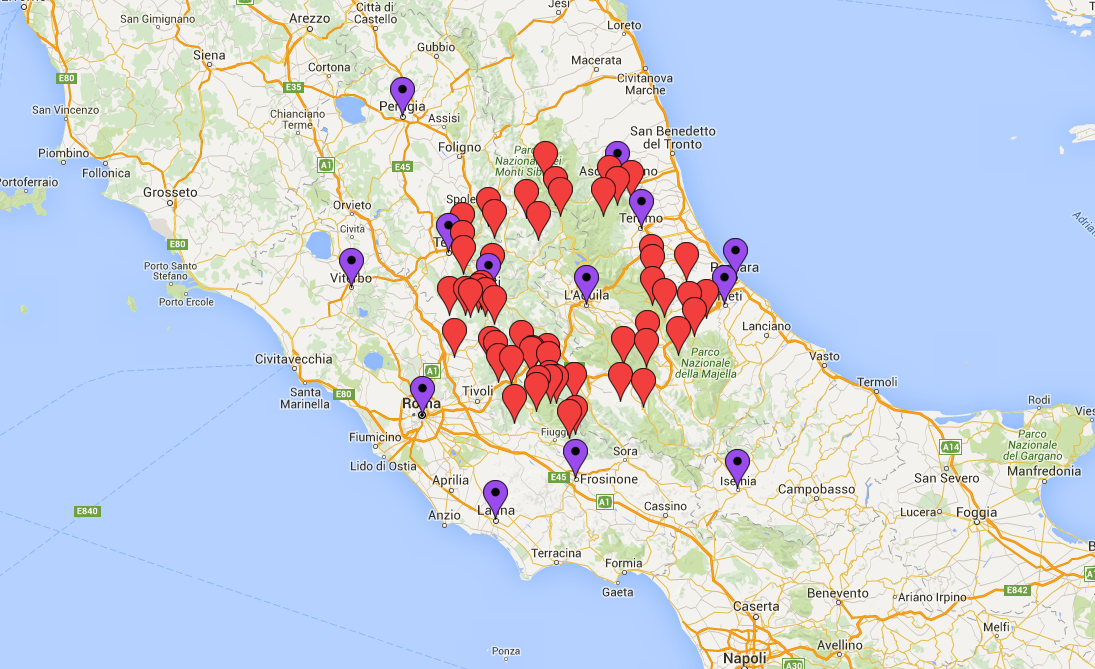
\includegraphics[keepaspectratio=true,height=200pt]{simulazione}

\end{frame}
\begin{frame}
	\frametitle{SeismoCloud: app per cellulari}
	
	\begin{itemize}
		\item Android, iOS
		\item Gratuita, presente nei canali ufficiali di distribuzione
		\item Contribuisce al rilevamento dei terremoti analizzando le vibrazioni (quando è poggiato su un tavolo)
		\item Riceve le notifiche di Early Warning
	\end{itemize}
	
\end{frame}
\begin{frame}
	\frametitle{SeismoCloud: il sismometro fisso}
	
	\begin{itemize}
		\item Schede principali: Intel Galileo, Raspberry PI + un accelerometro
		\item Sorgente libero e aperto (FOSS)
		\item Sistema operativo GNU/Linux
		\item Istruzioni sulla costruzione e funzionamento sul sito www.seismocloud.com
	\end{itemize}
	
	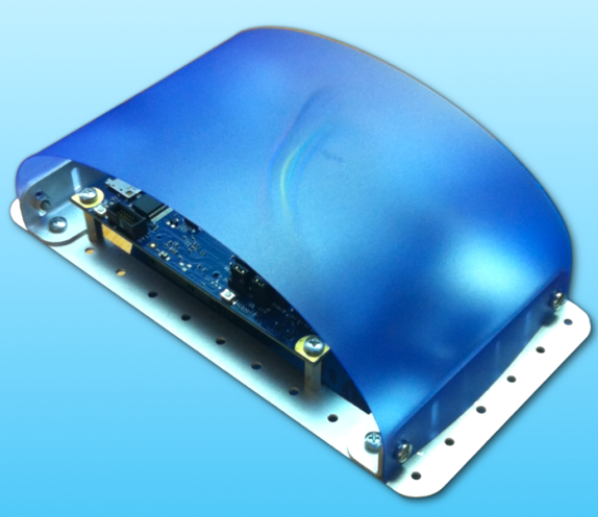
\includegraphics[keepaspectratio=true,width=100pt]{galileo}
	
\end{frame}


	\begin{frame}
		\frametitle{\hfill}
		
		\LARGE Domande?		
		
	\end{frame}
	
\end{document}
